\documentclass[11pt,a4paper]{report}
\usepackage[portuges]{babel}
\usepackage[utf8]{inputenc} 
\usepackage{graphicx} 
\usepackage{url} 
\usepackage{enumerate} 
\usepackage{color} 
\usepackage{textcomp}
\usepackage{indentfirst}
\usepackage{array} 
\usepackage{parskip}
\usepackage[export]{adjustbox}
\usepackage{xpatch}
\usepackage{amsmath}
\newlength{\chaptertopskip}
\setlength{\chaptertopskip}{10pt}
\usepackage{listings}


\usepackage{a4wide}
\usepackage{float}
\usepackage{minted}
\usepackage{multicol}
\usepackage{appendix}
\setlength{\parskip}{1em}
\usepackage{verbatim}

\usepackage[demo]{graphicx}
\usepackage{caption}
\usepackage{subcaption}




\usepackage[pdftex]{hyperref} 

\definecolor{saddlebrown}{rgb}{0.55, 0.27, 0.07}

\usepackage{listings}  

\lstset{
	basicstyle=\small, 
	numbers=left,
	numberstyle=\tiny, 
	numbersep=5pt,
	breaklines=true, 
    frame=tB,  
	mathescape=true,
	escapeinside={(*@}{@*)}
}

\usepackage{xspace}

\parindent=20pt 
\parskip=10pt 

\setlength{\oddsidemargin}{-1cm} 
\setlength{\textwidth}{18cm} 
\setlength{\headsep}{0cm} 
\setlength{\textheight}{23cm} 
\renewcommand{\baselinestretch}{1.5cm}




\setlength{\parskip}{1em}
\title{Guia de Utilização\\
	\large NECChange}

\author{Hugo Filipe de Sá Rocha  \\ (A96463) \and Miguel Ângelo Alves de Freitas \\ (A91635)         \and Simão Quintela\\ (A97444)
       } %autores do documento


\date{\today} %data

\begin{document}
	\begin{minipage}{0.9\linewidth}
        \centering
		
\includegraphics[width=0.4\textwidth]{um_lcc.jpg}\par\vspace{1cm}
		\href{https://www.uminho.pt/PT}
		{\scshape\LARGE Universidade do Minho} \par
		\vspace{0.6cm}
		\href{https://lcc.di.uminho.pt}
		{\scshape\Large Licenciatura em Ciências da Computação} \par
		\maketitle
	\end{minipage}

	
	\tableofcontents
	
	\pagebreak
	
	\chapter{Instalação de dependências}
 Antes de usar o programa pela primeira vez, devem ser instaladas as depêndencias necessárias para o bom funcionamento do mesmo.  
 
 Dependências necessárias:  

 \begin{itemize}
     \item Python 
     \item Poetry
     \item Node.js
 \end{itemize}

 \section{Windows e macOS}
\subsection{Python}
Python foi a linguagem escolhida para o back-end do programa. \\

Para a instalação do \href{https://www.python.org/downloads/}{Python} pode ser consultada a documentação oficial da linguagem.
 
 \subsection{Poetry}
Esta ferramenta é usada para gestão de dependências em Python de forma a que as mesmas fiquem encapsuladas no seu próprio ambiente para que o utilizador tenha mais facilidade ao dar setup ao programa.  \\

Para a instalação do \href{https://python-poetry.org/docs/#installing-with-the-official-installer}{Poetry} pode ser consultada a documentação oficial da ferramenta.

 \subsection{Node.js}
 O Node é uma ferramenta open-source que nos permite executar código em Javascript.\\

 Para a instalação do \href{https://nodejs.org/en/download}{Node.js} pode ser consultada a documentação oficial da ferramenta
 
 \section{Linux}.
 Em Linux a instalação destas ferramentas tornam-se imediatas, pelo qual vão ser listados os comandos a executar para diferentes package managers.  \\

\begin{verbatim}
Pacman 
    $ sudo pacman -Sy python-pip
    $ pip install poetry 
    $ sudo pacman -S nodejs npm

Apt
    $ sudo apt install python3
    $ pip install poetry
    $ sudo apt install nodejs
 
\end{verbatim}



\chapter{Setup inicial do programa}
Considerando que todas as ferramentas estão instaladas, para correr o programa é preciso fazer um setup inicial ao mesmo. Os passos a seguir são todos \textbf{executados no terminal} e são os seguintes:  \\

\textbf{1- Navegar até à diretoria Projeto/schedule} \\

\textbf{2- Inserir o comando poetry install } \\

\textbf{3- Navegar até à diretoria Projeto/web} \\

\textbf{4- Inserir o comando npm install} \\

Após estes 4 passos o setup fica concluído e não precisa de ser repetido em futuras utilizações. 

 
\chapter{Execução do programa}

Neste projeto há duas formas de execução do programa. \\ 

\textbf{1- Executar diretamente no back-end com geração de horários e acesso a um menu de estatísticas.} \\

\textbf{2- Executar o front-end onde pode ser feito o upload de ficheiros, geração, visualização e alteração de horários.} \\



\section{Ativar o Ambiente Virtual}
Em cada um dos casos é preciso fazer um passo de importância extrema, \textbf{ativar o ambiente virtual}. \\

\textbf{Nota: } Os seguintes passos, tanto em \textbf{Windows} como em \textbf{Linux}, apenas são necessários na primeira vez, desde que se guarde o comando a executar visto que será sempre o mesmo.

\subsection{Windows}
Para ativar o ambiente virtual em Windows temos de seguir os seguintes passos: \\

\textbf{1- Navegar até à diretoria Projeto/schedule}\\ 

\textbf{2- Executar o comando poetry env info}\\

O output esperado após este comando (varia dependendo da máquina e do sistema operativo) deve ser parecido com o seguinte:  \\

\begin{verbatim}
Virtualenv
Python:         3.11.1
Implementation: CPython
Path:           C:\Users\Utilizador\AppData\Local\Packages\PythonSoftwareFoundation.Python.3.11_qbz5n2kfra8p0\LocalCache\Local\pypoetry\Cache\virtualenvs\schedule-HT8ZFRxr-py3.11
Executable:     C:\Users\Utilizador\AppData\Local\Packages\PythonSoftwareFoundation.Python.3.11_qbz5n2kfra8p0\LocalCache\Local\pypoetry\Cache\virtualenvs\schedule-HT8ZFRxr-py3.11\Scripts\python.exe
Valid:          True

System
Platform:   win32
OS:         nt
Python:     3.11.1
Path:       C:\Users\Utilizador\AppData\Local\Microsoft\WindowsApps\PythonSoftwareFoundation.Python.3.11_3.11.496.0_x64__qbz5n2kfra8p0
Executable: python
\end{verbatim} \\ 

Copiamos agora o path que aparece na 5ª linha "Executable" e substituímos o último programa "python.exe" por "Activate". \\

Após a substituição, cola esse novo path no terminal, pressiona Enter e o ambiente virtual é ativado. \\

\subsection{Linux}
Para ativar o ambiente virtual em Linux temos de seguir os seguintes passos: \\

\textbf{1- Navegar até à diretoria Projeto/schedule}\\ 

\textbf{2- Executar o comando poetry env info}\\
O output esperado após este comando (varia dependendo da máquina e do sistema operativo) deve ser parecido com o seguinte:  \\

\begin{verbatim}
Virtualenv
Python:         3.10.10
Implementation: CPython
Path:           /home/{nome_do_utilizador}/.cache/pypoetry/virtualenvs/schedule-UP-QV2il-py3.10
Valid:          True

System
Platform: linux
OS:       posix
Python:   /usr
\end{verbatim} \\ 

Copiamos agora o path que aparece na 4ª linha "Path" e executa-se no terminal o seguinte comando:  \\
\textbf{source pathQueFoiCopiado/bin/activate}  \\



\section{Executar o programa}
Com o ambiente virtual ativo estamos em condições de correr o nosso programa: \\

\textbf{Caso 1 - Executar diretamente o Back-end} \\

1- Navegar até à diretoria Projeto/schedule/schedule \\ 

2- Executar o comando python main.py

\textbf{Caso 2 - Executar o Front-end} \\

1- Navegar até à diretoria Projeto/web \\ 

2- Executar o comando npm run dev

3- Navegar no browser até http://localhost:3000
 
\chapter{Carregamento de ficheiros}
Já na página do servidor local, no lado esquerdo encontra-se a secção \textbf{Upload}. Aqui, devem ser carregados três ficheiros no formato \textbf{.csv}. 

\begin{itemize}
  \item O primeiro ficheiro deve conter a informação do horário de cada Unidade Curricular (UC) do curso.
  \item O segundo ficheiro deve conter a informação sobre a inscrição dos alunos nas respetivas UCs.
  \item O terceiro ficheiro deve conter informação sobre a capacidade de cada sala.
\end{itemize}

Após carregar os ficheiros, ao clicar no botão \textbf{Upload}, estes são carregados para o servidor. A aplicação fornece feedback ao utilizador: em caso de sucesso, uma notificação verde com a mensagem "Upload successful!" é apresentada; em caso de erro, uma notificação vermelha é exibida com a respetiva mensagem de erro.

Por fim, o utilizador pode solicitar a geração do novo horário ao clicar no botão \textbf{Generate}. Este botão inicia a execução do algoritmo que processa os dados carregados e gera o novo horário. Similarmente ao processo de upload, o utilizador é informado do sucesso ou falha da operação através de uma notificação.

\begin{figure}[H]
    \centering
    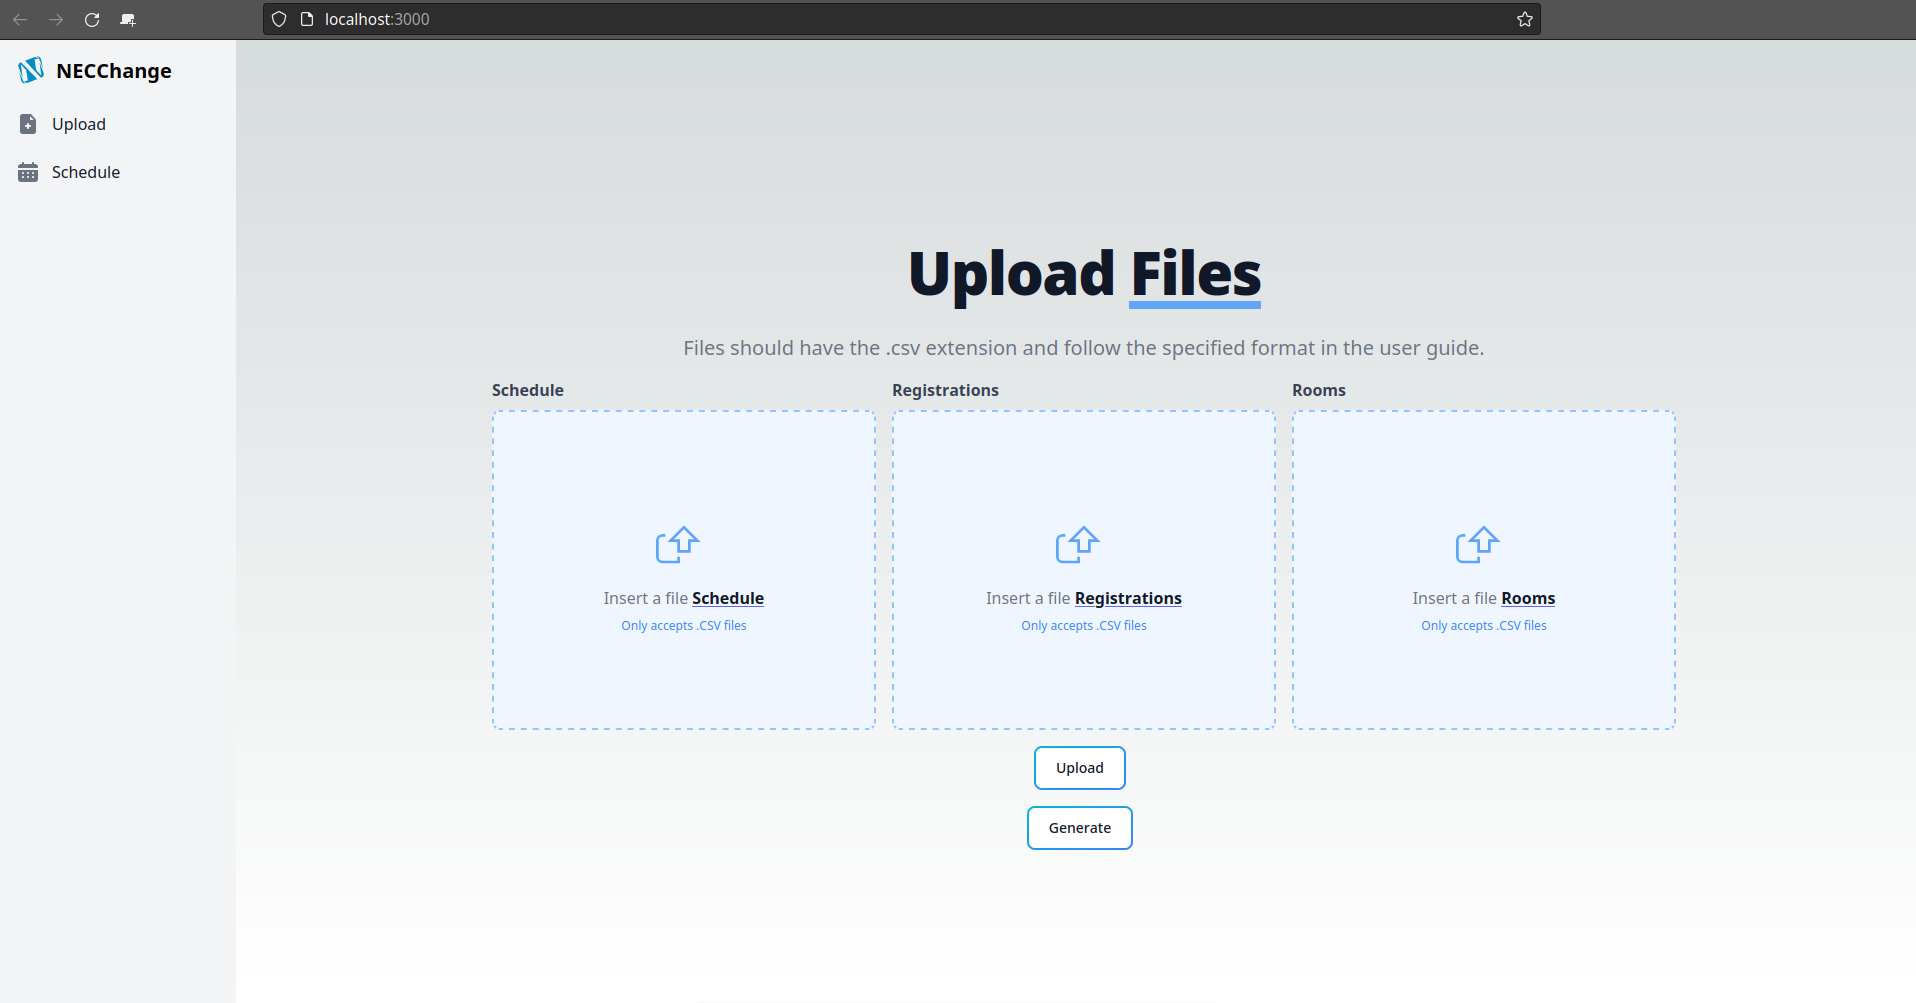
\includegraphics[width=0.8\textwidth,height=0.8\textheight,keepaspectratio]{upload.png}
    \caption{\texttt{Página de upload}}
\end{figure}

    
    \pagebreak
    \chapter{Visualização dos horários}
Para visualizar os horários gerados, clica-se na separador \textbf{Schedule}, do lado esquerdo, onde podemos consultar o horário gerado para cada aluno, colocando o respetivo número mecanográfico. Após isso, apenas é necessário clicar em \textbf{Search} e o horário do aluno será disponibilizado graficamente. Para melhor compreensão do horário, foi colocada uma cor acizentada nos slots onde existem sobreposições de aulas. Além disso, as cadeiras de diferentes anos possuem diferentes cores, nomeadamente, às unidades curriculares do primeiro ano ficou associada a cor azul, às de segundo a cor vermelha e, por fim, as disciplinas do último ano ficaram com a cor verde.


    \pagebreak
    \chapter{Troca de turnos}
A troca de turnos para um dado aluno deve ser feita também na secção \textbf{Schedule}, do lado esquerdo. Para um dado aluno, ao clicarmos no botão \textbf{Trades} conseguimos obter todas as unidades curriculares onde o aluno está inscrito, podendo alterar o seu turno diretamente, clicando no botão \textbf{Submit}.

    \begin{center}
    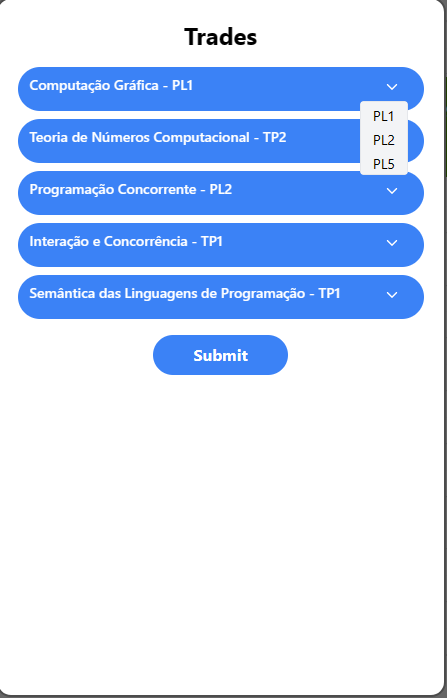
\includegraphics[scale=0.5]{trades.png}
    \caption{Secção trades}
    \end{center}
    \vskip 50
    

\end{document}